% !TEX root = task-4-3-3.tex
% Editable task bank. Append new BankTask blocks at the end of the document.
\documentclass[12pt,a4paper]{article}
\usepackage{physics-textbook}
\usepackage{graphicx,needspace}
\usetikzlibrary{decorations.pathmorphing}
\newif\ifShowSolutions
\ifdefined\TutorEdition
  \ShowSolutionstrue
\else
  \ShowSolutionsfalse % Change to \ShowSolutionstrue to display solutions.
\fi
\newcounter{banktask}
\newsavebox{\BankTaskBox}
\newcommand{\BankTaskContent}[3]{%
  \noindent\textbf{\thebanktask.}\quad #2\par
  \ifShowSolutions
    \Needspace{50mm}% Keep the solution heading with its opening text or diagram.
    #3\par
    \ifdefined\TutorEdition
      \ifcsname TutorSource#1\endcsname
        \nopagebreak\smallskip{\small\csname TutorSource#1\endcsname\par}%
      \fi
    \fi
  \fi
}
\newcommand{\BankTask}[3]{%
  \refstepcounter{banktask}\par\medskip
  \sbox{\BankTaskBox}{\begin{minipage}{\linewidth}%
    \BankTaskContent{#1}{#2}{#3}\end{minipage}}%
  \ifdim\dimexpr\ht\BankTaskBox+\dp\BankTaskBox\relax>\dimexpr\textheight-20mm\relax
    \Needspace{35mm}\BankTaskContent{#1}{#2}{#3}%
  \else
    \Needspace{\dimexpr\ht\BankTaskBox+\dp\BankTaskBox\relax}%
    \noindent\usebox{\BankTaskBox}\par
  \fi
  \medskip
}
\begin{document}
\BookSubsection{4.3.3}{Закон преломления (общий случай)}


% Source 209C4E: https://ege.fipi.ru/bank/questions.php?search=1&proj=BA1F39653304A5B041B656915DC36B38&qid=209C4E
\BankTask{209C4E}{
Школьник, изучая законы геометрической оптики, провёл опыт по преломлению света (см. рисунок). Для этого он направил узкий пучок света на стеклянную пластину.
\begin{center}
\begin{tabular}{|c|c|c|c|c|}
\hline
Угол $\alpha$ & $20^\circ$ & $40^\circ$ & $50^\circ$ & $70^\circ$ \\
\hline
$\sin\alpha$ & $0{,}34$ & $0{,}64$ & $0{,}78$ & $0{,}94$ \\
\hline
\end{tabular}
\end{center}
\begin{enumerate}
\item Угол падения равен $70^\circ$.
\item Показатель преломления стекла примерно равен $1{,}47$.
\item Угол преломления равен $50^\circ$.
\item Наблюдается полное внутреннее отражение.
\item Угол отражения равен $20^\circ$.
\end{enumerate}
\begin{center}
\begin{tikzpicture}[book diagram,scale=1.15]
\fill[gray!35] (0,0) circle (2.1);
\shade[top color=gray!60,bottom color=white] (-1.56,0) arc[start angle=180,end angle=360,radius=1.56]--cycle;
\draw (-1.56,0)--(1.56,0) arc[start angle=0,end angle=-180,radius=1.56];
\draw (0,0) circle (2.1);
\foreach \a in {0,5,...,355}{\draw (\a:1.98)--(\a:2.1);}
\foreach \a in {0,10,...,350}{\draw (\a:1.88)--(\a:2.1);}
\foreach \a in {0,30,...,330}{\draw (\a:1.81)--(\a:2.1);}
\node[rotate=90] at (0:1.72) {$0$};
\node[rotate=60] at (30:1.72) {$30$};
\node[rotate=30] at (60:1.72) {$60$};
\node at (90:1.72) {$90$};
\node[rotate=-30] at (120:1.72) {$60$};
\node[rotate=-60] at (150:1.72) {$30$};
\node[rotate=90] at (180:1.72) {$0$};
\node[rotate=60] at (210:1.72) {$30$};
\node[rotate=30] at (240:1.72) {$60$};
\node[rotate=180] at (270:1.72) {$90$};
\node[rotate=-30] at (300:1.72) {$60$};
\node[rotate=-60] at (330:1.72) {$30$};
\draw[thick] (0,0)--(0,1.56);
\draw[gray!80,very thick,-{book tip}] (160:2.9)--(160:2.13);
\draw[white,line width=0.9pt] (160:2.1)--(0,0)--(20:2.1);
\draw[gray!80,very thick,-{book tip}] (20:2.1)--(20:2.9);
\draw[white,line width=1.5pt] (0,0)--(-50:2.1);
\draw[gray!80,line width=0.5pt] (0,0)--(-50:2.1);
\draw[gray!80,very thick,-{book tip}] (-50:2.1)--(-50:2.9);
\end{tikzpicture}
\end{center}
}{
\smallskip\noindent\textbf{Решение от GPT}\par
Угол падения отсчитывают от нормали: $\alpha=90^\circ-20^\circ=70^\circ$, поэтому утверждение 1 верно. Угол преломления $\beta=90^\circ-50^\circ=40^\circ$, а показатель преломления стекла $n=\sin70^\circ/\sin40^\circ=0{,}94/0{,}64\approx1{,}47$: утверждение 2 верно, утверждение 3 неверно. Преломлённый луч присутствует, поэтому полного внутреннего отражения нет и утверждение 4 неверно. Угол отражения равен углу падения, то есть $70^\circ$, поэтому утверждение 5 неверно. Ответ: 1, 2.
}

% Source 626E20: https://ege.fipi.ru/bank/questions.php?search=1&proj=BA1F39653304A5B041B656915DC36B38&qid=626E20
\BankTask{626E20}{
Пучок монохроматического света переходит из стекла в воздух. Длина волны света в воздухе — \(\lambda\); скорость света в воздухе — \(c\); показатель преломления стекла относительно воздуха — \(n\).

Установите соответствие между физическими величинами и формулами, по которым их можно рассчитать.

\begin{center}
\TaskMatchingColumns[0.56\linewidth]{Физические величины}{
А) частота света в воздухе\par
Б) скорость света в стекле
}{Формулы}{
1) \(\dfrac{c}{\lambda}\)\par
2) \(\dfrac{n\cdot\lambda}{c}\)\par
3) \(\dfrac{n\cdot c}{\lambda}\)\par
4) \(\dfrac{c}{n}\)
}
\end{center}

\begin{center}
\begin{tabular}{|c|c|}
\hline
А & Б \\
\hline
\phantom{1} & \phantom{4} \\
\hline
\end{tabular}
\end{center}
}{
\smallskip\noindent\textbf{Решение от GPT}\par
Частота света в воздухе определяется равенством \(c=\lambda\nu\), откуда \(\nu=c/\lambda\) (1). По определению относительного показателя преломления \(n=c/v_{\text{ст}}\), поэтому скорость света в стекле \(v_{\text{ст}}=c/n\) (4). Формула 2 имеет размерность времени, а формула 3 даёт \(n\nu\), поэтому они не подходят. Ответ: \(\boxed{14}\).
}

% Source AE8774: https://ege.fipi.ru/bank/questions.php?search=1&proj=BA1F39653304A5B041B656915DC36B38&qid=AE8774
\BankTask{AE8774}{
Пучок монохроматического света переходит из воды в воздух. Скорость света в воде — \(\upsilon\); скорость света в воздухе — \(c\); длина световой волны в воде — \(\lambda\). Установите соответствие между физическими величинами и формулами, по которым их можно рассчитать.

\begin{center}
\TaskMatchingColumns[0.56\linewidth]{Физические величины}{
А) длина световой волны в воздухе\par
Б) показатель преломления воды относительно воздуха
}{Формулы}{
1) \(\dfrac{\upsilon}{c}\)\par
2) \(\dfrac{c}{\upsilon}\)\par
3) \(\dfrac{\upsilon\cdot\lambda}{c}\)\par
4) \(\dfrac{\lambda\cdot c}{\upsilon}\)
}
\end{center}

\begin{center}
\begin{tabular}{|c|c|}
\hline
А & Б \\
\hline
\phantom{4} & \phantom{2} \\
\hline
\end{tabular}
\end{center}
}{
\smallskip\noindent\textbf{Решение от GPT}\par
Частота при переходе света через границу сред сохраняется: \(\nu=\upsilon/\lambda\), поэтому длина волны в воздухе \(\lambda_{\text{возд}}=c/\nu=\lambda c/\upsilon\) (4). Показатель преломления воды относительно воздуха равен \(n=c/\upsilon\) (2). Формула 1 даёт обратный показатель преломления, а формула 3 ошибочно уменьшает длину волны при переходе в воздух, поэтому они не подходят. Ответ: \(\boxed{42}\).
}

% Source 154E79: https://ege.fipi.ru/bank/questions.php?search=1&proj=BA1F39653304A5B041B656915DC36B38&qid=154E79
\BankTask{154E79}{
Необходимо собрать экспериментальную установку, с помощью которой можно определить показатель преломления стекла. Для этого школьник взял источник света, создающий узкий пучок света, карандаш и циркуль. Какие два предмета из приведённого ниже перечня оборудования необходимо дополнительно использовать для проведения этого эксперимента?
\begin{enumerate}
\item плоскопараллельная стеклянная пластина
\item линейка
\item плоскопараллельная плексигласовая пластина
\item зеркало
\item собирающая линза
\end{enumerate}
}{
\smallskip\noindent\textbf{Решение от GPT}\par
Нужны стеклянная пластина (1) и линейка (2): отмечают ход луча, строят нормаль к границе и с помощью циркуля и линейки определяют отношение \(n=\sin\alpha/\sin\beta\), считая показатель преломления воздуха равным единице. Плексигласовая пластина (3) позволяет исследовать другой материал, зеркало (4) даёт отражение, а собирающая линза (5) не нужна для измерения углов на плоской границе стекла. Ответ: 1, 2.
}

% Source 16868: https://phys-ege.sdamgia.ru/problem?id=16868
\BankTask{16868}{
\begin{center}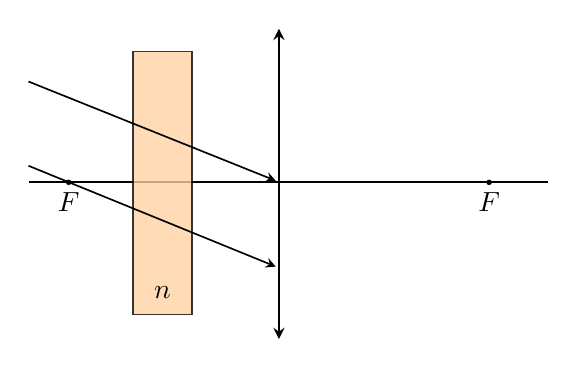
\begin{tikzpicture}[>=stealth,line width=.6pt]

\draw(-3.18,0)--(3.42,0);
\draw[<->,thick](0,-1.99)--(0,1.95);
\fill(-2.67,0)circle(.035) (2.67,0)circle(.035);
\node[below]at(-2.67,0){$F$};\node[below]at(2.67,0){$F$};
\draw[fill=orange!36,opacity=.78](-1.85,-1.68)rectangle(-1.10,1.66);\node at(-1.48,-1.4){$n$};\draw[->](-3.18,1.28)--(-.04,.02);\draw[->](-3.18,.21)--(-.04,-1.07);
\end{tikzpicture}\end{center}
На тонкую собирающую линзу от удаленного источника падает пучок параллельных лучей (см. рис.). Как изменится положение изображения источника, создаваемого линзой, если между линзой и ее фокусом поставить плоскопараллельную стеклянную пластинку с показателем преломления n (на рисунке положение пластинки отмечено пунктиром)? Ответ поясните, указав, какие физические закономерности Вы использовали. Сделайте рисунок, поясняющий ход лучей до и после установки плоскопараллельной стеклянной пластинки.
}{
\smallskip\noindent\textbf{Решение}\par
Построим изображение в линзе до и после установки плоскопараллельной пластинки. Для построения изображения пользуемся следующими соображениями. Луч, проходящий через центр линзы проходит непреломленным. Параллельный пучок света собирается в фокальной плоскости линзы.
После установки плоскопараллельной пластинки луч света будет преломляться внутри нее, но на выходе получим пучок света параллельный исходному. Поясним это соображение. По закону Снеллиуса оптические плотности сред n$_{1}$, n$_{2}$, угол падения $\alpha_{1}$, угол преломления $\alpha_{2}$, связаны соотношением: $n_1 \sin \alpha _1 = n_2 \sin \alpha _2.$ При выходе из пластины закон Снеллиуса также выполняется, получаем: $n_1 \sin \alpha _1 = n_2 \sin \alpha _2 = n_1 \sin \alpha _3.$ То есть синусы падающего и выходящего лучей равны, а значит, равны и углы под которыми, соответственно, падают и выходят эти лучи.


\begin{center}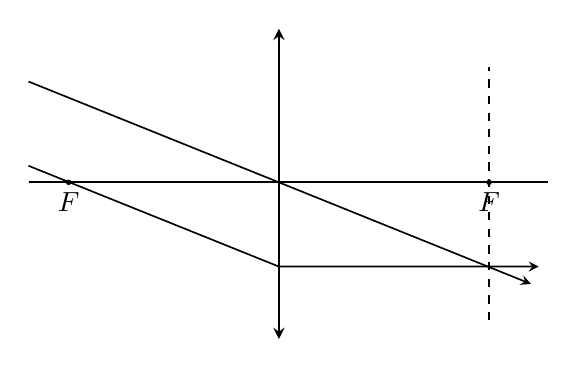
\begin{tikzpicture}[>=stealth,line width=.6pt]

\draw(-3.18,0)--(3.42,0);
\draw[<->,thick](0,-1.99)--(0,1.95);
\fill(-2.67,0)circle(.035) (2.67,0)circle(.035);
\node[below]at(-2.67,0){$F$};\node[below]at(2.67,0){$F$};
\draw[dashed](2.67,-1.75)--(2.67,1.47);\draw[->](-3.18,1.28)--(0,0)--(3.20,-1.29);\draw[->](-3.18,.21)--(0,-1.07)--(3.30,-1.07);
\end{tikzpicture}\end{center}



\begin{center}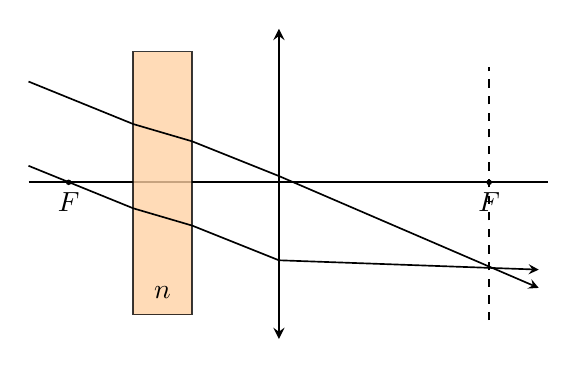
\begin{tikzpicture}[>=stealth,line width=.6pt]

\draw(-3.18,0)--(3.42,0);
\draw[<->,thick](0,-1.99)--(0,1.95);
\fill(-2.67,0)circle(.035) (2.67,0)circle(.035);
\node[below]at(-2.67,0){$F$};\node[below]at(2.67,0){$F$};
\draw[fill=orange!36,opacity=.78](-1.85,-1.68)rectangle(-1.10,1.66);\node at(-1.48,-1.4){$n$};\draw[dashed](2.67,-1.75)--(2.67,1.47);\draw[->](-3.18,1.28)--(-1.85,.74)--(-1.10,.52)--(0,.08)--(3.30,-1.341);\draw[->](-3.18,.21)--(-1.85,-.33)--(-1.10,-.55)--(0,-.99)--(3.30,-1.109);
\end{tikzpicture}\end{center}


Таким образом, получаем, что положение изображения источника после установки плоскопараллельной пластинки не изменится.
}

% Source 29157: https://phys-ege.sdamgia.ru/problem?id=29157
\BankTask{29157}{
\begin{center}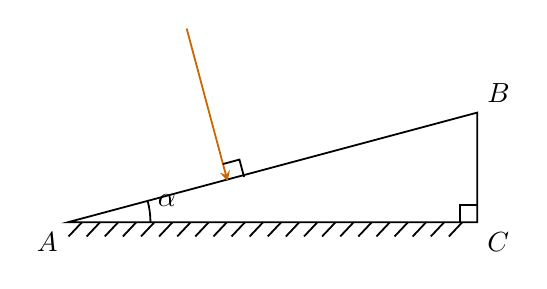
\begin{tikzpicture}[>=stealth,line width=.65pt]\draw (0,0)--(5.2,0)--(5.2,1.393)--cycle;\draw (1.05,0)arc(0:15:1.05)node[right]{$\alpha$};\foreach \x in {.18,.41,...,5.2}{\draw(\x,0)--++(-.17,-.18);}\draw (4.98,0)--(4.98,.22)--(5.2,.22);\draw[->,orange!80!black] (1.51,2.46)--(2.03,.52);\draw (1.971,.74)--(2.18,.796)--(2.239,.576);\node[below left]at(0,0){$A$};\node[above right]at(5.2,1.393){$B$};\node[below right]at(5.2,0){$C$};\end{tikzpicture}\end{center}

Нижняя грань AC прозрачного клина посеребрена и представляет собой плоское зеркало. Угол при вершине клина $\alpha = 15\ensuremath{{}^{\circ}}.$ Луч света падает из воздуха на клин перпендикулярно грани AB, преломляется и выходит в воздух через ту же грань AB, но уже под углом преломления $\beta = 60\ensuremath{{}^{\circ}}.$ Определите показатель преломления клина. Сделайте рисунок, поясняющий ход луча в клине.
}{
\smallskip\noindent\textbf{Решение}\par
\begin{center}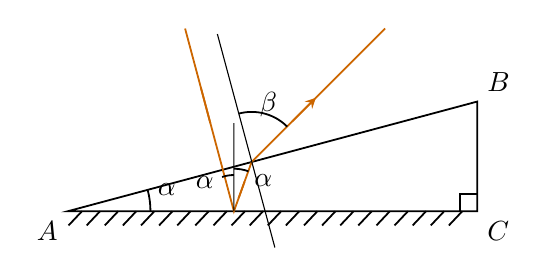
\begin{tikzpicture}[>=stealth,line width=.65pt]\draw (0,0)--(5.2,0)--(5.2,1.393)--cycle;\draw (1.05,0)arc(0:15:1.05)node[right]{$\alpha$};\foreach \x in {.18,.41,...,5.2}{\draw(\x,0)--++(-.17,-.18);}\draw (4.98,0)--(4.98,.22)--(5.2,.22);\draw[orange!80!black] (1.49,2.32)--(2.11,0)--(2.335,.626)--(4.03,2.32);\draw[->,orange!80!black](1.69,1.57)--(1.81,1.12) (2.17,.168)--(2.245,.375) (2.85,1.14)--(3.15,1.44);\draw[thin](2.11,0)--(2.11,1.12) (1.9,2.25)--(2.63,-.46);\draw (2.11,.46)arc(90:109:.46) (2.11,.54)arc(90:70:.54);\node[left]at(1.98,.37){$\alpha$};\node[right]at(2.24,.39){$\alpha$};\draw (2.17,1.24)arc(105:45:.638)node[above left]{$\beta$};\node[below left]at(0,0){$A$};\node[above right]at(5.2,1.393){$B$};\node[below right]at(5.2,0){$C$};\end{tikzpicture}\end{center}

$1$.  Луч, падающий на грань АВ, не преломляется, так как угол падения равен $0$\ensuremath{{}^{\circ}}. При падении на зеркальную грань $AC$ он падает под углом, который из геометрических соображений равен углу $\alpha .$ По закону отражения света угол отражения будет также равен $\alpha .$ 
$2$.  Данный луч падает на грань АВ под углом $\alpha _1=2 \alpha .$ По закону преломления света $\frac{\sin \alpha _1}{\sin \beta} = \frac{1}{n} ,$ откуда показатель преломления материала клина 

\[n= \frac{\sin \beta}{\sin 2 \alpha} = \frac{\sin 60 ^\circ}{\sin ( 2 \cdot 15 ^\circ )} = \sqrt{3} \approx 1{,}73.\]

Ответ: $1{,}73$.
}

\end{document}
